\documentclass{article}
\usepackage[utf8]{inputenc}
\title{MATH 20C Notes - Week Three}
\author{C-Rin}
\date{October 2019}

\usepackage{natbib}
\usepackage{graphicx}
\usepackage{gensymb}
\usepackage{amsmath}
\usepackage{amssymb}

\usepackage{diffcoeff}


\graphicspath{ {./images/} }

\begin{document}

\maketitle

\section*{Introduction}
Deep 

\begin{figure}[h!]
\centering

\includegraphics[scale=0.09]{crab.jpg}
\caption{A crab}
\end{figure}

\section{Limits and Continuity}
In 1D, $f: \mathbb{R}\rightarrow\mathbb{R}$, and 

\[\lim_{\vec{v}\rightarrow\vec{a}}\vec{f}(\vec{v})=\vec{b}\]
if $\vec{f}(\vec{v})$ gets arbitrarily close to $\vec{b}$ as $\vec{v}$ approaches $\vec{a}$ (close means the distance $||\vec{f}(\vec{v})-\vec{b}||$ is small).

\subsection{Precise Definition}
\[\mbox{Say}\lim_{\vec{v}\rightarrow\vec{a}}\vec{f}(\vec{v})=\vec{b}\]
if for all $\epsilon\leq 0$ there exists $\delta\ge 0$ such that whenever $||\vec{v}-\vec{a}||\le\delta$, then $||\vec{f}(\vec{v})-\vec{b}||\le\epsilon$

\subsection{Properties of Limits}
Suppose $\lim_{\vec{v}\rightarrow\vec{a}}\vec{f}(\vec{v})=\vec{b}$ and $\lim_{\vec{v}\rightarrow\vec{a}}\vec{g}(\vec{v})=\vec{c}$ and $f:\mathbb{R}^n\rightarrow\mathbb{R}^m$
\begin{enumerate}
    \item $\lim_{\vec{v}\rightarrow\vec{a}}\vec{f}(\vec{v})+\vec{g}(\vec{v})=\vec{b}+\vec{c}$
    \item If $\lambda$ is a real number, then $\lim_{\vec{v}\rightarrow\lambda\vec{a}}\vec{f}(\vec{v})=\lambda\vec{b}$
    \item $f(x_1,\ldots,x_n)=\overbrace{(f_{1}(x_1,\ldots,x_n),\ldots,f_{m}(x_1,\ldots,x_n))}^{m different real valued functions}$
\end{enumerate}

$\lim_{\vec{v}\rightarrow\vec{a}}\vec{f}(\vec{v})=\vec{b}=(b_1,\dots,b_n)$ if and only if $\lim_{\vec{v}\rightarrow\vec{a}}\vec{f}_i(\vec{v})=\vec{b}_i$ for all $1\leq i\leq m$

A function is \textbf{continuous} if for any $\vec{a}$, we have $\lim_{\vec{v}\rightarrow\vec{a}}\vec{f}(\vec{v})=\vec{f}(\vec{a})$

\subsubsection*{Nonexample}

Consider $f:\mathbb{R}^2\rightarrow\mathbb{R}$ to be $(x,y)\rightarrow\frac{x^2}{x^2+y^2}$\\
What is the limit of $f(x,y)$?\\
To understand the question, we take sections from the function.

For $x=0$
\[f(0,y)=\frac{0}{0+y^2}=0\;\; \mbox{ When $y\neq0$}\]
\[\mbox{So }\lim_{y\rightarrow0}f(0,y)=0\]
For $y=0$
\[f(x,0)=\frac{x^2}{x^2+0}=1\]
\[\mbox{So }\lim_{x\rightarrow0}f(x,0)=1\]
For $x=y$
\[f(x,x)=\frac{x^2}{x^2+x^2}=\frac{x^2}{2x^2}=\frac{1}{2}\]
\[\mbox{So }\lim_{x\rightarrow0}f(x)=\frac{1}{2}\]

\subsubsection*{Example}
\[f(x,y)=\frac{2x^{2}y}{x^2+y^2}\]
$x$ Section
\[f(0,y)=\frac{0}{y^2}=0\]
$y$ Section
\[f(x,0)=\frac{0}{x^2}=0\]
$x=y$ Section
\[\lim_{(x,y)\rightarrow(0,0)}f(x,x)=\frac{2x^{2}y}{x^2+y^2}=0\]

\subsection{Properties of Continuous Functions}

\begin{itemize}
    \item Polynomial functions are continuous
    \[f(x,y,z)=(x^3+xyz+z^3)\]
    \item Compositions of two continuous functions are continuous
    \[f: \mathbb{R}^n\rightarrow\mathbb{R}^m\]
    \[g: \mathbb{R}^m\rightarrow\mathbb{R}^p\]
    \[\mbox{if $f$ and $g$ are continuous, then $g\cdot f$ is continuous.}\]
    \item Sums of $\overbrace{\mbox{continuous functions}}^{\mbox{or scalar multiples}}$ are continuous 
    \item $f: \mathbb{R}^m\rightarrow\mathbb{R}^n$
    \[(x_1,\ldots,x_m)\rightarrow f(x_1,\ldots,x_m)=(f_1(x_1,\ldots,x_m),\ldots,f_n(x_1,\ldots,x_m))\]
\end{itemize}
$f$ is continuous if and only if all the $f_i$s are continuous.
\[f:\mathbb{R}\rightarrow\mathbb{R}^2\]
\[t\rightarrow(\overbrace{t}^{f_1(t)},\overbrace{t^2}^{f_2(t)})\]

\section{Differentiation}
\[f:\mathbb{R}^m\rightarrow\mathbb{R}^n\]
\[\frac{\partial f}{\partial x}\mathbb{R}^3\rightarrow\mathbb{R}\]
What is the meaning of the derivative?

\subsection{Partial Derivative}
$\frac{\partial f}{\partial x}$ is the partial derivative with respect to x.
\[f:\mathbb{R}^3\rightarrow\mathbb{R}^1\;\;\;\mbox{for }(x,y,z)\]

\[\frac{\partial f}{\partial x}(x,y,z)=\lim_{h\rightarrow 0}\frac{f(x+h,y,z)-f(x,y,z)}{h}\]
\[\frac{\partial f}{\partial y}(x,y,z)=\lim_{h\rightarrow 0}\frac{f(x,y+h,z)-f(x,y,z)}{h}\]
\[\frac{\partial f}{\partial z}(x,y,z)=\lim_{h\rightarrow 0}\frac{f(x,y,z+h)-f(x,y,z)}{h}\]

\subsection{Tangent Planes}
As the derivative of a single variable function creates a tangent line, the derivative of a surface creates tangent planes.

\begin{figure}[h!]
    \centering
    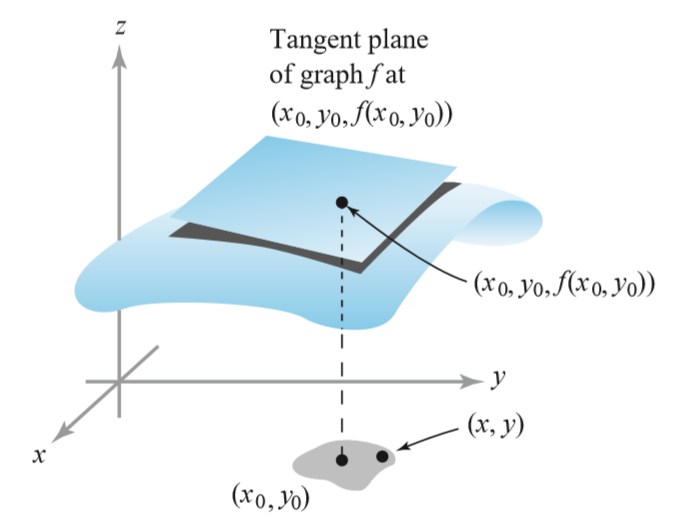
\includegraphics[scale=.5]{tangentPlaneDiff.png}
    \caption{}
    \label{}
\end{figure}

What is the relation between $\frac{\partial g}{\partial x}$ and $\frac{\partial g}{\partial y}$ and the tangent plane?\\

The graph of $f$ has two tangent vectors.
\[(1,0,\frac{\partial g}{\partial x},(x_o,y_o))\]
\[(0,1,\frac{\partial g}{\partial y},(x_o,y_o))\]

\subsection{Equation for the Tangent Plane}

\textbf{The Normal Vector}
\[\overbrace{\bar{n}=v_1\times v_2=(-\frac{\partial g}{\partial x}(x_o,y_o),-\frac{\partial g}{\partial y}(x_o,y_o),1)}^{\mbox{recovers the "slope" of the tangent plane}}\]

Looking at the section of $z=g$
\[\frac{\partial g}{\partial x}(x_o,y_o)=\lim_{h\rightarrow 0}\frac{g(x_{o}+h,y_o)-g(x_{o},y_{o})}{h}\]\\

\[\bar{n}\cdot (x-x_o,y-y_o,z-f(x_o,y_o))=0\]
\[z=g(x,y)+\frac{\partial g}{\partial x}(x-x_o)+\frac{\partial g}{\partial y}(y-y_o)\]
\[\mbox{Also called the linear approximation to $g$}\]

\subsection*{Example}
Compare the linear approximation to $z=x^2+y^4$ at $(x_o,y_o)=1,0$


\[\frac{\partial z}{\partial x}=2x+0=2x\qquad\;\;\; \frac{\partial z}{\partial y}=4y^3\]
\[\frac{\partial z}{\partial x}(1,0)=2\cdot 1=2\qquad \frac{\partial z}{\partial y}(1,0)=0\]
\[\bar{n}=(-2,0,1)\]
\[z=g(x_o,y_o)+2\cdot(x-1)+0(y-0)=1+2(x-1=2x-1)\]


\subsection*{Exercise}
Find the equation for the tangent plane to $z=x^2-y^{3}x$ at $(1,1)$

\[\frac{\partial z}{\partial x}=2x-y^3\qquad\;\;\; \frac{\partial z}{\partial y}=-3y^{2}x\]
\[\frac{\partial z}{\partial x}(1,1)=2-1=1\qquad \frac{\partial z}{\partial y}(1,1)=-3\]
\[\bar{n}=(-1,3,0)\]
\[z=g(x_o,y_o)+1\cdot (x-1)+(-3)(y-1)=0+x-1-3+3=x-3y+2\]
\[z=x-3y+2\]

\section{The Derivative of Multi-Variable Functions}

The derivative of $\vec{f}$ denoted by $D\vec{f}$ is the matrix
\[\textit{D}\vec{f}=
\begin{bmatrix}
    \frac{\partial f_1}{\partial x_1}(\vec{v})&\frac{\partial f_1}{\partial x_2}(\vec{v})&\ldots&\frac{\partial f_1}{\partial x_m}(\vec{v})\\[6pt]
    \frac{\partial f_2}{\partial x_1}(\vec{v})&\frac{\partial f_2}{\partial x_2}(\vec{v})&\ldots&\frac{\partial f_2}{\partial x_m}(\vec{v})\\[6pt]
    \vdots&\vdots&\ddots&\vdots\\[6pt]
    \frac{\partial f_n}{\partial x_1}(\vec{v})&\frac{\partial f_n}{\partial x_2}(\vec{v})&\ldots&\frac{\partial f_n}{\partial x_m}(\vec{v})
\end{bmatrix}\]

\subsection*{Example}
\[\vec{f}(x,y)=(\cos (xy),e^{xy})\]
\[\mbox{Domain: $\mathbb{R}^2$ Co-Domain: $\mathbb{R}^2$}\]
\[\vec{f}:\mathbb{R}^2 \rightarrow\mathbb{R}^2\]

Compute $D\vec{f}(1,1)$

\[D\vec{f}(1,1)=\begin{bmatrix}
    \frac{\partial f_1}{\partial x}(1,1)&\frac{\partial f_1}{\partial y}(1,1)\\[6pt]
    \frac{\partial f_2}{\partial x}(1,1)&\frac{\partial f_2}{\partial y}(1,1)
\end{bmatrix}\]



\begin{center}
    \begin{tabular}{ c c c }
     $f_{1}(x,y)=\cos (xy)$ & $\frac{\partial \vec{f}_1}{\partial x}=-y\sin (xy)$ & $\frac{\partial \vec{f}_2}{\partial y}=y e^x$ \\[6pt]
     
     $f_{2}(x,y)=e^{xy}$ & $\frac{\partial f_1}{\partial y}=-x\sin (xy)$ & $\frac{\partial f_2}{\partial y}=xe^{xy}$ 
    \end{tabular}
\end{center}

\[D\vec{f}(1,1)=\begin{bmatrix}
    -\sin (1\cdot 1)&-\sin (1\cdot 1)\\
    e^{1\cdot 1}& e^{1\cdot 1}
\end{bmatrix}=\begin{bmatrix}
    -\sin (1)&-\sin (1)\\
    e&e
\end{bmatrix}\]
    
\subsection*{Exercise}
$\vec{f}(t)=(1,2,3)+t(1,1,1)$\\[4pt]
Compute $D\vec{f}(0)$\\
Domain: $\mathbb{R}$ and Co-domain: $\mathbb{R}^3$

\[\vec{f}(t)=(1,2,3)+t(1,1,1)\]
\[\vec{f}(t)=(\overbrace{1+t}^{f_{1}(t)}\overbrace{2+t}^{f_{2}(t)},\overbrace{3+t}^{f_{3}(t)})\]

\[\begin{matrix}
    \frac{\partial f_1}{\partial t}=1& \frac{\partial f_2}{\partial t}=1& \frac{\partial f_3}{\partial t}=1
\end{matrix}\]
\[D\vec{f}=\begin{bmatrix}
    1\\
    1\\
    1
\end{bmatrix}\]
\newpage
\subsection{Definition}
\[f: \mathbb{R}^n\rightarrow\mathbb{R}\]
\textit{Df} is also denoted $\nabla f$ and called the gradient of \textit{f}.

If $f: \mathbb{R}^2\rightarrow\mathbb{R}$
\[\overbrace{z=f(x_o,y_o)+\frac{\partial f}{\partial x}(x_o,y_o)(x-x_o)+\frac{\partial f}{\partial y}(x_o,y_o)(y-y_o)}^{\mbox{Linear Approximation}}\]
\[\nabla f(x_o,y_o)=\begin{bmatrix}
    \frac{\partial f}{\partial x}(x_o,y_o)&\frac{\partial f}{\partial y}(x_o,y_o)
\end{bmatrix}\]
\[\overbrace{z=f(x_o,y_o)+\nabla f(x_o,y_o)\cdot (x-x_o,y-y_o)}^{\mbox{The same as linear approximation}}\]








\end{document}